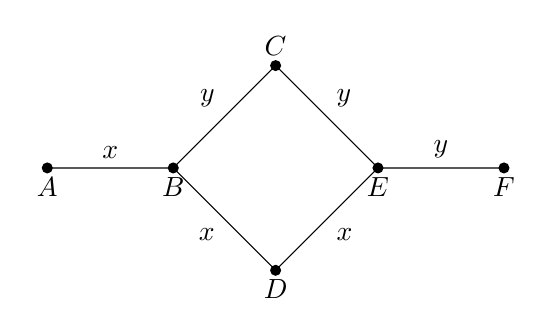
\begin{tikzpicture}
\coordinate (A) at (0,0); \coordinate (B) at (1.6,0); \coordinate (C) at (2.9,1.3); \coordinate (D) at (2.9,-1.3); \coordinate (E) at (4.2,0); \coordinate (F) at (5.8,0);
\draw (A) -- node[above]{$x$} (B) -- node[above left]{$y$} (C) -- node[above right]{$y$} (E) -- node[above]{$y$} (F);
\draw (B) -- node[below left]{$x$} (D) -- node[below right]{$x$} (E);
\foreach \p/\a in {A/below,B/below,C/above,D/below,E/below,F/below} { \fill (\p) circle (2pt); \node[\a] at (\p) {$\p$}; }
\end{tikzpicture}
